\section{Backlog Maintenance}

Managing Backlogs
\newline\newline
Backlogs can be easily maintained. Creating a backlog is the exact same process as creating any other type of model (via the File menu or the \'+\' button). Once you have opened the create window the only two things necessary for the creation of a backlog are the short name and the PO assigned to the backlog.
\newline
Adding a new story to a back log is easy. Simply select it from the story drop down (optionally give it a priority) and then press add. Prioritised stories will appear in the top of the table, ordered by their priority. Unprioritised stories will appear below them. To change the priority of a story simply select it and click on the up and down arrows to the side of the table. To remove a story simply click the X next to it.

\begin{figure}[H]
\centering
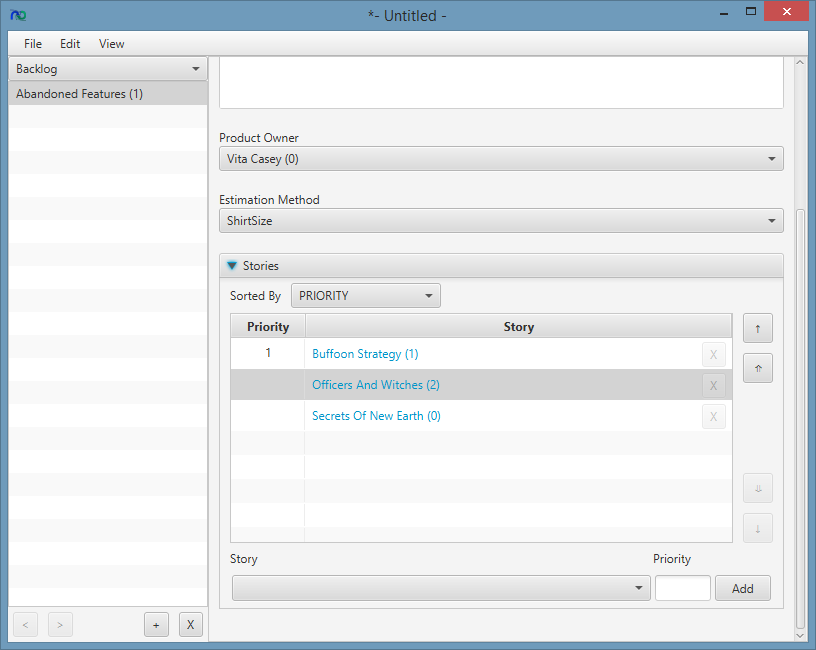
\includegraphics[width=\textwidth]{images/screenshots/backlogs.PNG}
\caption{The Backlogs Edit Pane}
\label{fig:new_project}
\end{figure}

\newline
Estimation Methods
\newline
Changing the estimation method changes how you estimate the difficulty of stories within the backlog. The supported types are Fibonacci (1,2,3,5,8,13), ShirtSizes (XS,S,M,L,XL,XXXL) and Movie Ratings (PG,G,M,R16,R18,Banned). You can change this at any time and the program will do its best to convert to the new scale.

\begin{figure}[H]
\centering
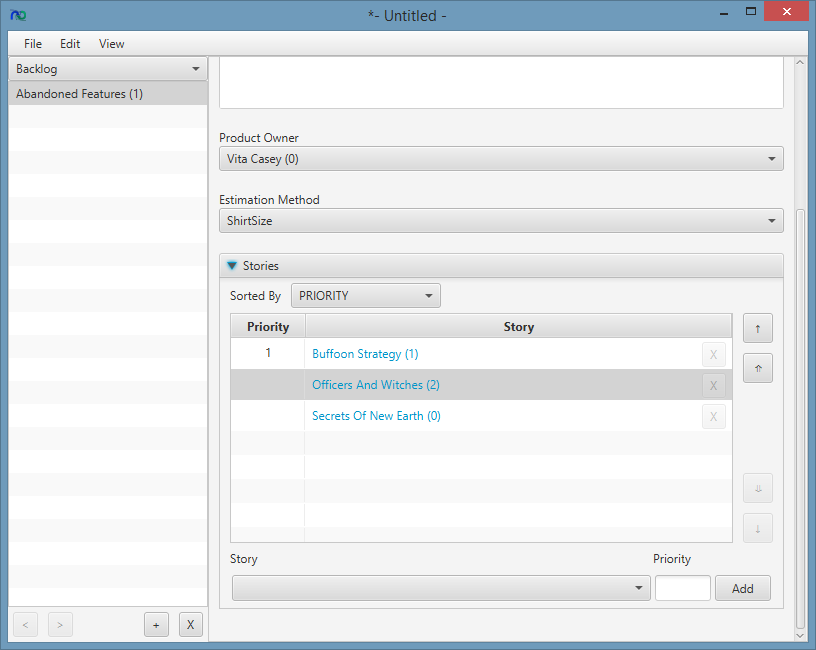
\includegraphics[width=\textwidth]{images/screenshots/backlogs.PNG}
\caption{The Estimate Method Choicebox}
\label{fig:new_project}
\end{figure}